\appendix

\chapter{Full Requirements List}\label{sec:requirements}

\begin{table}[htbp]
    \centering
    \begin{tabular}{|c|p{10cm}|c|}
    \hline
    \textbf{ID}  & \textbf{Requirement}  & \textbf{Priority} \\ \hline
    2.1  & The system must provide a secure login mechanism for patients by using a combination of login and password. & Must Have \\ \hline
    2.2 & The system should provide an option for password recovery. & Should Have \\ \hline
    \end{tabular}
    \caption{Login Requirements}
\end{table}
    
\begin{table}[htbp]
    \centering
    \begin{tabular}{|c|p{10cm}|c|}
    \hline
    \textbf{ID}  & \textbf{Requirement}  & \textbf{Priority} \\ \hline
    4.1  & The system must allow the patient to generate a shareable link to provide access to their medical records. & Must Have \\ \hline
    4.2  & When creating the shareable link, the system must allow the patient to set an expiration date for the link. & Must Have \\ \hline
    4.3  & When creating the shareable link, the system should allow the patient to set an access PIN for the link. & Should Have \\ \hline
    4.4  & When creating the shareable link, the system should allow the patient to select which records to share with the doctor. & Should Have \\ \hline
    \end{tabular}
    \caption{Patient Shareable Link Requirements}
\end{table}

\begin{table}[htbp]
    \centering
    \begin{tabular}{|c|p{10cm}|c|}
    \hline
    \textbf{ID}  & \textbf{Requirement}  & \textbf{Priority} \\ \hline
    1.1  & The system must be accessible on all modern desktop and mobile-based browsers. & Must Have \\ \hline
    1.2  & The system must protect sensitive data through encryption at rest and in transit. & Must Have \\ \hline
    1.3 & The system must hash and salt all passwords before storing them in the database. & Must Have \\ \hline
    1.4 & The system must encrypt uploaded documents before storing them in the file system. & Must Have \\ \hline
    1.5 & The system must allow access only to the patient's associated records. & Must Have \\ \hline
    1.6 & When records are shared, the system must allow a doctor's access only to the selected shared records. & Must Have \\ \hline  
    1.7 & The system must provide clear error messages to users when operations fail or errors occur during data entry. & Must Have \\ \hline
    1.8 & The system must be able to handle file uploads of at least 10MB and support multiple file formats (PDF, DOC, etc). & Must Have \\ \hline
    1.9 & The web application should have a responsive design that adapts to different screen sizes. & Should Have \\ \hline
    1.10 & The application should have a consistent design across all pages & Should Have \\ \hline
    1.11 & The system interface should be available in the Romanian language & Should Have \\ \hline
    1.12  & When shared with the doctor via a link, the share link must load within 3 to 5 seconds. & Should Have \\ \hline
    1.13 & The system should validate the share link using its expiration time and PIN before allowing access. & Could Have \\ \hline
    \end{tabular}
    \caption{Non-functional Requirements}
\end{table}

\begin{table}[htbp]
    \centering
    \begin{tabular}{|c|p{10cm}|c|}
    \hline
    \textbf{ID}  & \textbf{Requirement}  & \textbf{Priority} \\ \hline
    3.1  & The system must allow patients to upload their own medical records in a variety of formats (PDF, DOC, etc). & Must Have \\ \hline
    3.2 & The system should allow to upload files/documents for other types of records (vaccine certificates, etc). & Should Have \\ \hline
    3.2  & The system must allow the patient to specify and categorise the type of document they are uploading (lab test, doctor consultation, etc). & Must Have \\ \hline
    3.3 & When a the lab category is selected during record creation, the system must allow the user to enable AI processing. & Must Have \\ \hline
    3.4 & If lab extraction was enabled, the system must display the extraction results to the user before sending to the database. & Must Have \\ \hline
    3.5 & The system must allow the patient to add a description of the document they are uploading. & Must Have \\ \hline
    3.6 & The system should allow the patient to add a date for the document they are uploading. & Should Have \\ \hline
    3.7 & The system should allow the patient to add a location for the document they are uploading. & Should Have \\ \hline
    3.8 & The system should allow the patient to add the doctor name for the document they are uploading. & Should Have \\ \hline
    3.9 & The system should allow the patient to sort and filter the documents based on the type of document, date, location, and doctor name. & Should Have \\ \hline
    3.10 & If used on mobile, the system should allow the patient to take a picture of the document and upload it. & Could Have \\ \hline
    \end{tabular}
    \caption{Document Upload Requirements}
\end{table}

\begin{table}[htbp]
    \centering
    \begin{tabular}{|c|p{10cm}|c|}
    \hline
    \textbf{ID}  & \textbf{Requirement}  & \textbf{Priority} \\ \hline
    5.1  & The patient personal cabinet must provide an overview of the patient's history through 3 main sections: personal information, lab tests, and doctor consultations. & Must Have \\ \hline
    5.2  & The system must display the patient's history in a chronological order in a table format. & Must Have \\ \hline
    5.3 & The system must have a dashboard view which displays an overview of the most recent information added to the system (latest lab tests, doctor consultations, vaccinations etc). & Must Have \\ \hline
    5.4  & The system must allow patients to add their own personal information, such as name or date of birth. & Must Have \\ \hline
    5.5  & The system must allow the patient to add their own allergies. & Must Have \\ \hline
    5.6  & The system must allow the patient to add their own vaccinations. & Must Have \\ \hline
    5.7  & When viewing doctor consultations, the system should divide them into categories based on the domain of the doctor (cardiology, neurology, etc). & Should Have \\ \hline
    5.8  & The system should allow the patient to enter vitals information, such as height, weight, blood pressure, etc. & Should Have \\ \hline
    5.9  & The system should display the information in both a list or grid view. & Should Have \\ \hline
    5.10  & When multiple vital and lab entries are made, the system should display a historical graph of the patient's vitals. & Should Have \\ \hline
    5.11 & The system should allow the patient to switch between viewing the lab tests in the document format or in a tabular, numerical format. & Should Have \\ \hline
    \end{tabular}
    \caption{Patient Personal Cabinet Requirements}
\end{table}

\begin{table}[htbp]
    \centering
    \begin{tabular}{|c|p{10cm}|c|}
    \hline
    \textbf{ID}  & \textbf{Requirement}  & \textbf{Priority} \\ \hline
    6.1  & The system must provide an overview of the patient history through 3 main sections: personal information, lab tests, and doctor consultations. & Must Have \\ \hline
    6.2  & When shared with the doctor, the system must allow the doctor to only view the patient's history, not edit it. & Must Have \\ \hline
    6.3  & The system must allow the doctor to view blood tests in a graphical format. & Must Have \\ \hline
    6.4  & The system must allow the doctor to view blood tests in a numerical, tabular format. & Must Have \\ \hline
    6.5  & The system must allow the doctor to view the patient's history in a chronological order. & Must Have \\ \hline
    6.6  & The system must display the doctor consultation and every lab test, except for blood tests, in a free text or document format. & Must Have \\ \hline
    6.7  & When viewing blood test results, the system should show the source document of the blood test value. & Should Have \\ \hline
    6.8  & For blood test results, the system should display the normal range values for each test. & Should Have \\ \hline
    \end{tabular}
    \caption{Shared Patient Information Requirements (Doctor View)}
\end{table}

\begin{table}[htbp]
    \centering
    \begin{tabular}{|c|p{10cm}|c|}
    \hline
    \textbf{ID}  & \textbf{Requirement}  & \textbf{Priority} \\ \hline
    7.1  & The system must allow patients to enter their current medication including details such as the name of the drug, dosage, frequency and start/end date. & Must Have \\ \hline
    7.2 & The system must allow patients to add new medication to their list. & Must Have \\ \hline
    7.3  & The system could allow patients to set medication reminders. & Should Have \\ \hline
    7.4 & After entering the medication, the system could allow the patient to track the medication intake. & Could Have \\ \hline

    \end{tabular}
    \caption{Patient Medication Requirements}
\end{table}

\chapter{Full Wireframes List}\label{sec:wireframes}

\begin{figure}[ht]
    \centering
    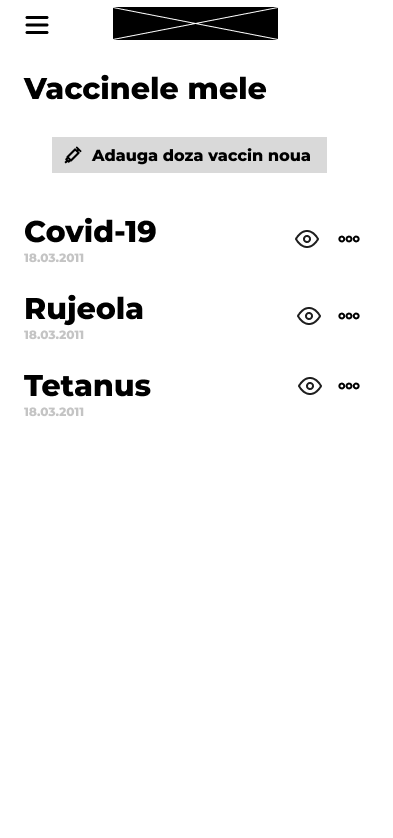
\includegraphics[width=0.3\textwidth]{wireframes/Mobile_vaccines.png}
    \caption{Mobile version of the Vaccines screen}
\end{figure}

\begin{figure}[ht]
    \centering
    \subfloat[Desktop version]{%
        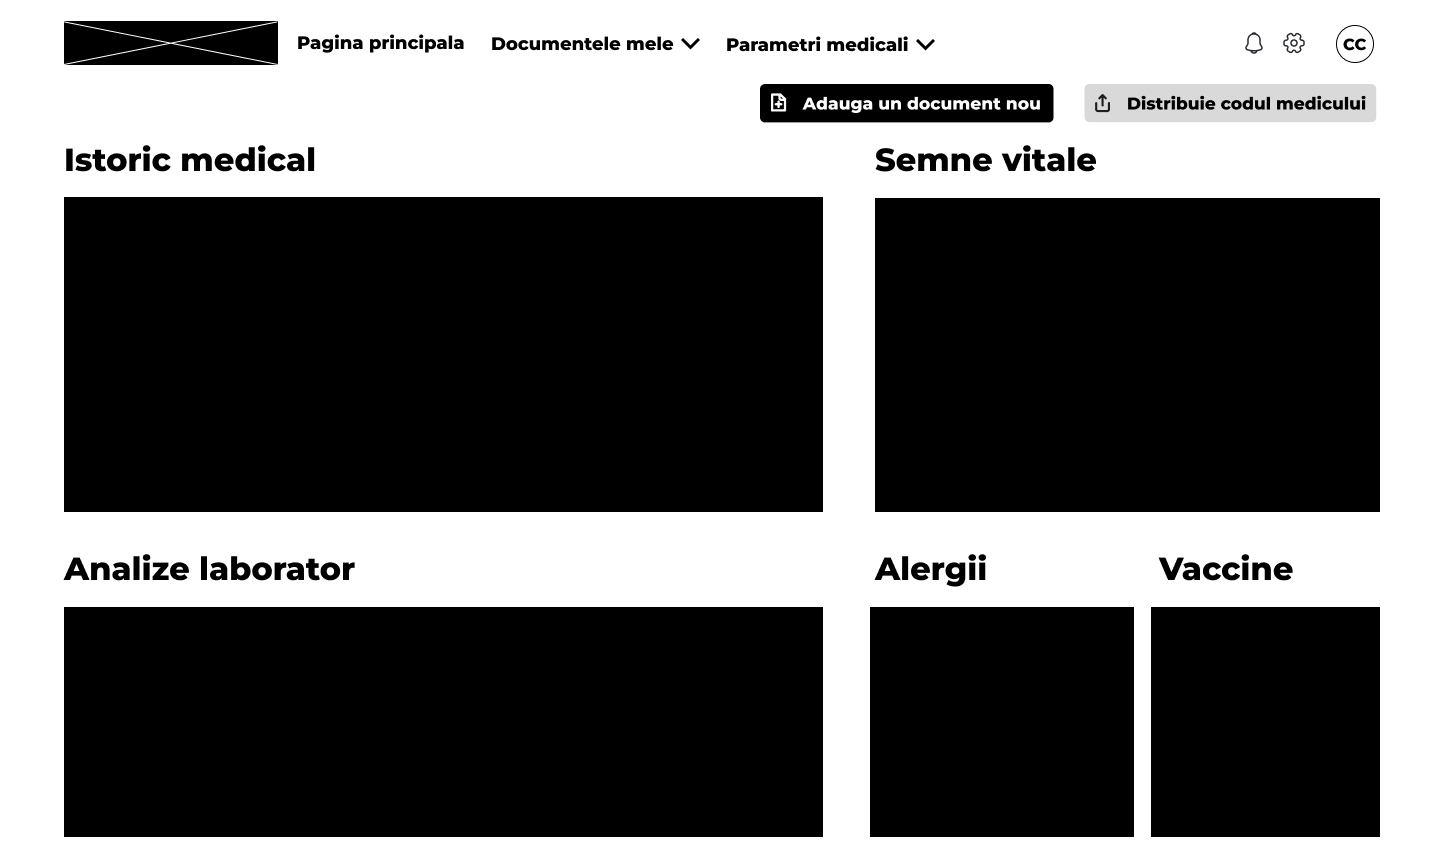
\includegraphics[width=0.75\textwidth]{wireframes/Desktop_dashboard.png}%
    }
    \hspace{0.05\textwidth}
    \subfloat[Mobile version]{%
        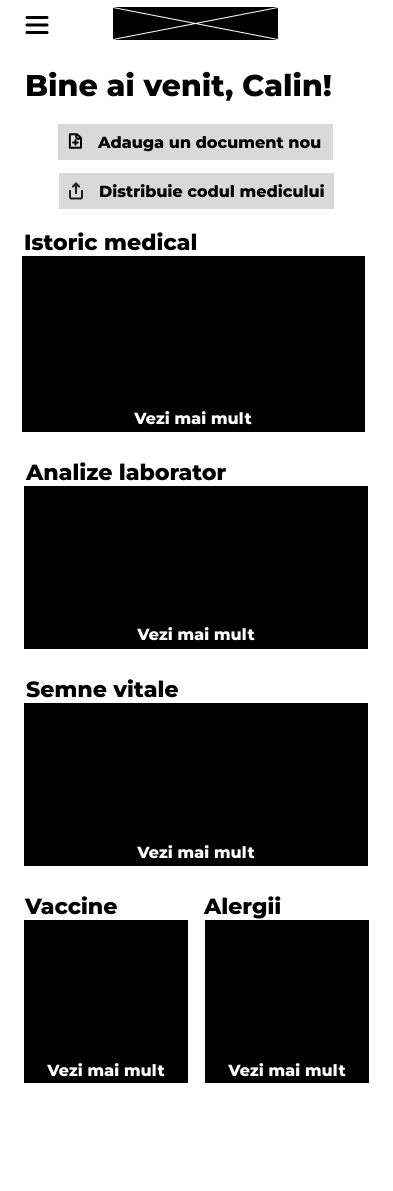
\includegraphics[scale=0.25]{wireframes/Mobile_dashboard.png}%
    }
    \caption{Desktop and Mobile version of the Dashboard screen}
\end{figure}

\begin{figure}[ht]
    \centering
    \subfloat[Desktop version]{%
        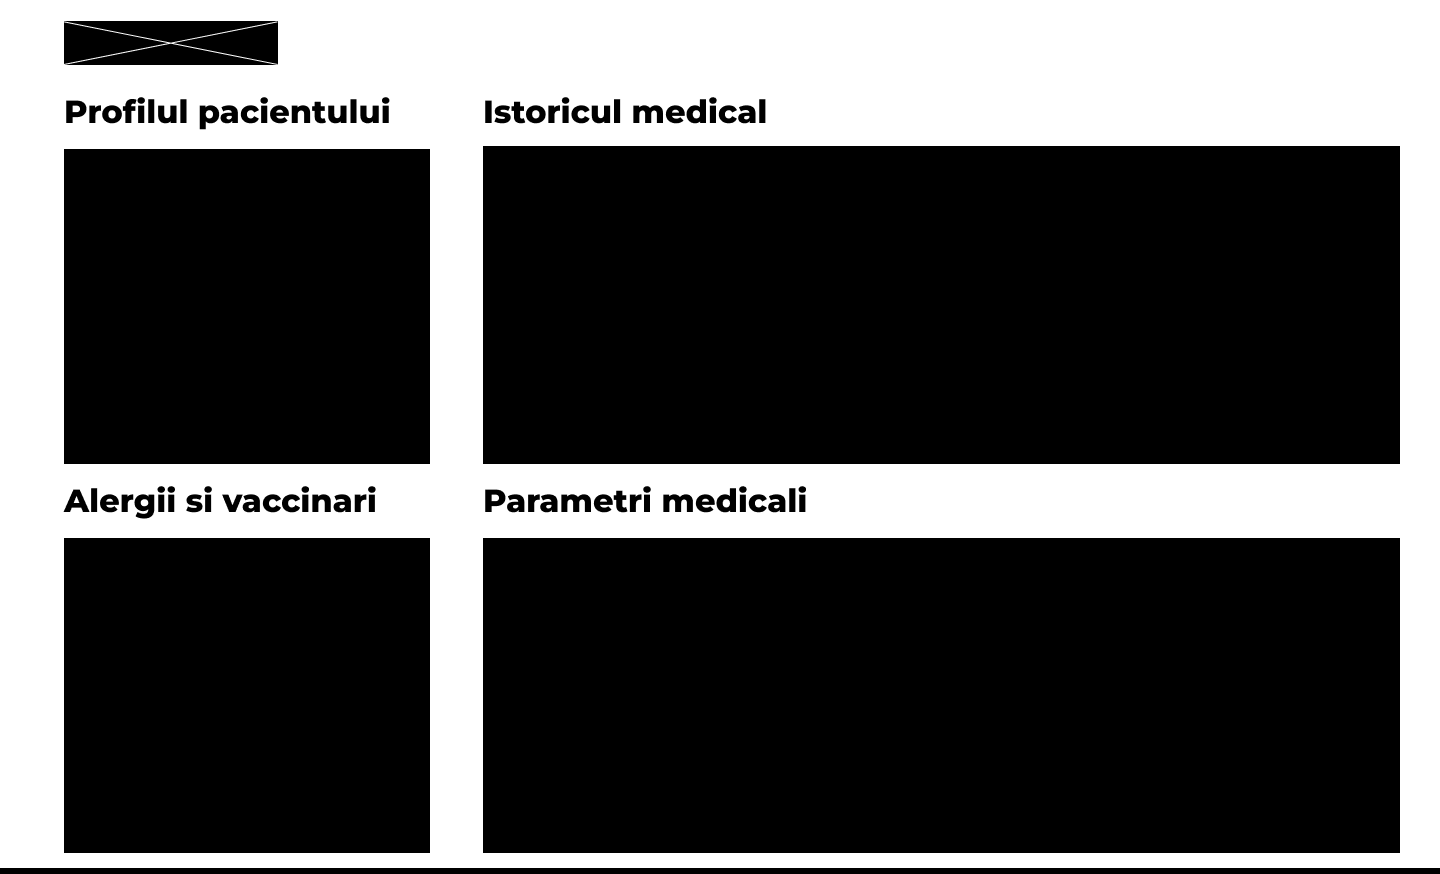
\includegraphics[width=0.75\textwidth]{wireframes/Desktop_doctorView.png}%
    }
    \hspace{0.05\textwidth}
    \subfloat[Mobile version]{%
        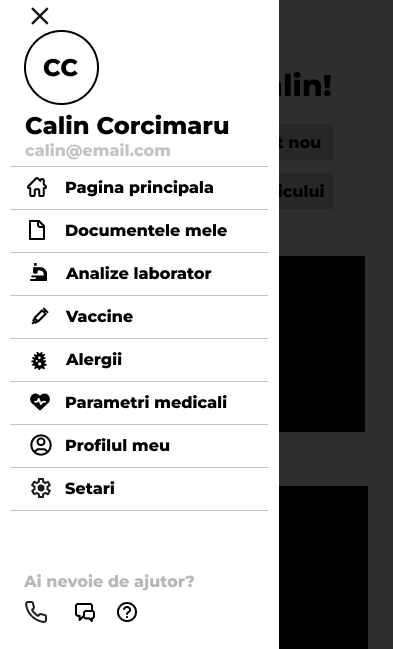
\includegraphics[scale=0.3]{wireframes/Mobile_dashboardMenu.png}%
    }
    \caption{Desktop and Mobile version of the Doctor View screen}
\end{figure}

\begin{figure}[ht]
    \centering
    \subfloat[Desktop version]{%
        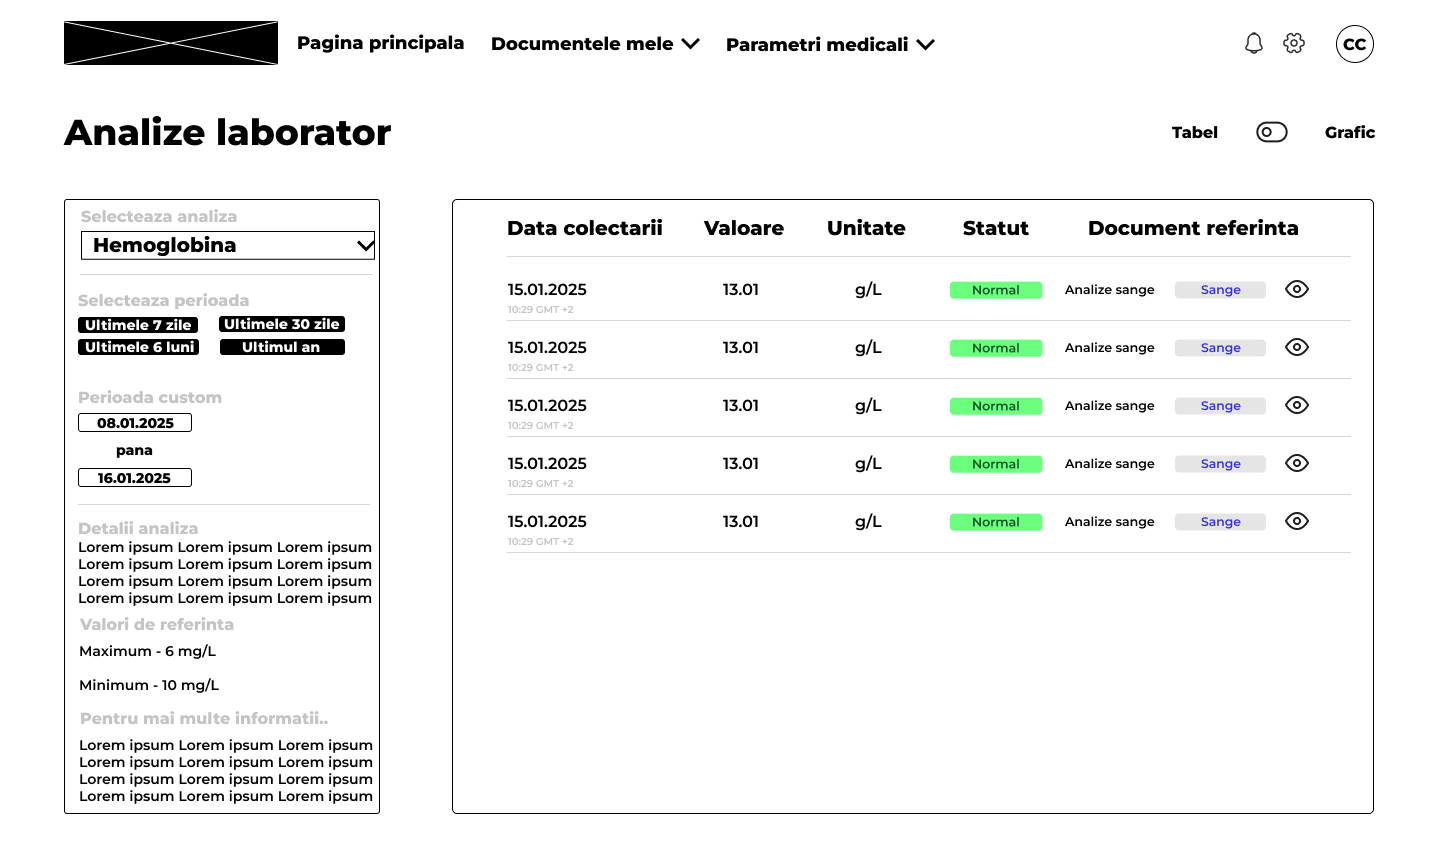
\includegraphics[width=0.75\textwidth]{wireframes/Desktop_labTest.png}%
    }
    \hspace{0.05\textwidth}
    \subfloat[Mobile version]{%
        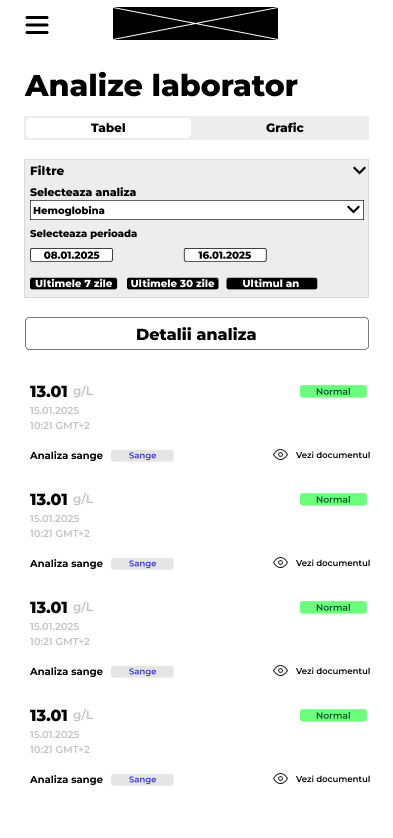
\includegraphics[scale=0.3]{wireframes/Mobile_labTest.png}%
    }
    \caption{Desktop and Mobile version of the Lab Test screen}
\end{figure}

\begin{figure}[ht]
    \centering
    \subfloat[Desktop version]{%
        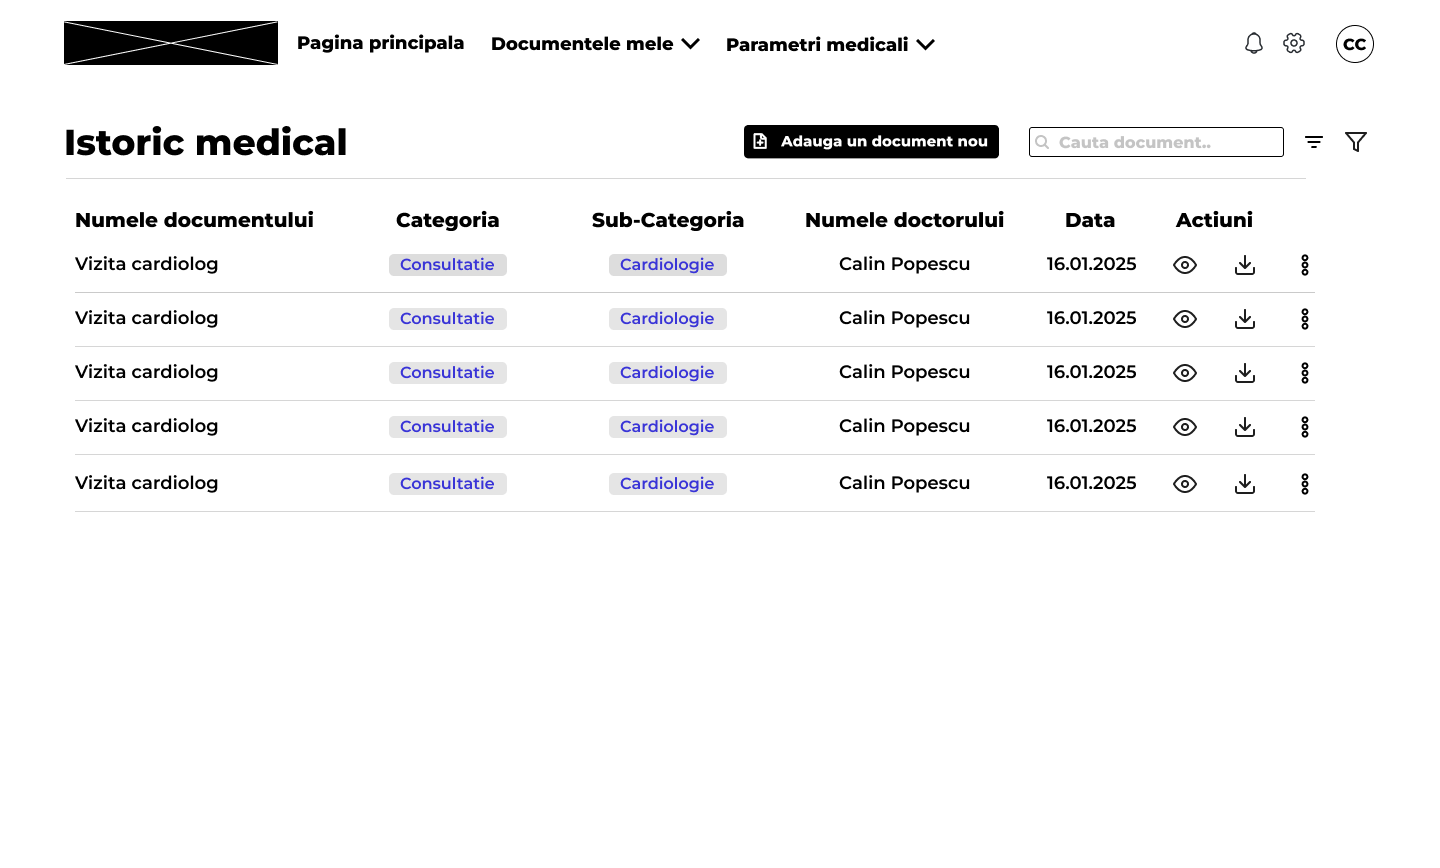
\includegraphics[width=0.75\textwidth]{wireframes/Desktop_medHistory.png}%
    }
    \hspace{0.05\textwidth}
    \subfloat[Mobile version]{%
        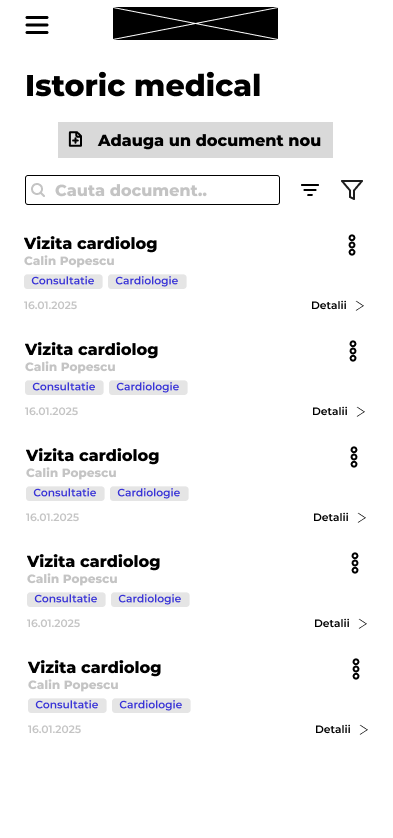
\includegraphics[scale=0.3]{wireframes/Mobile_medHistory.png}%
    }
    \caption{Desktop and Mobile version of the Medical History screen}
\end{figure}

\begin{figure}[ht]
    \centering
    \subfloat[Desktop version]{%
        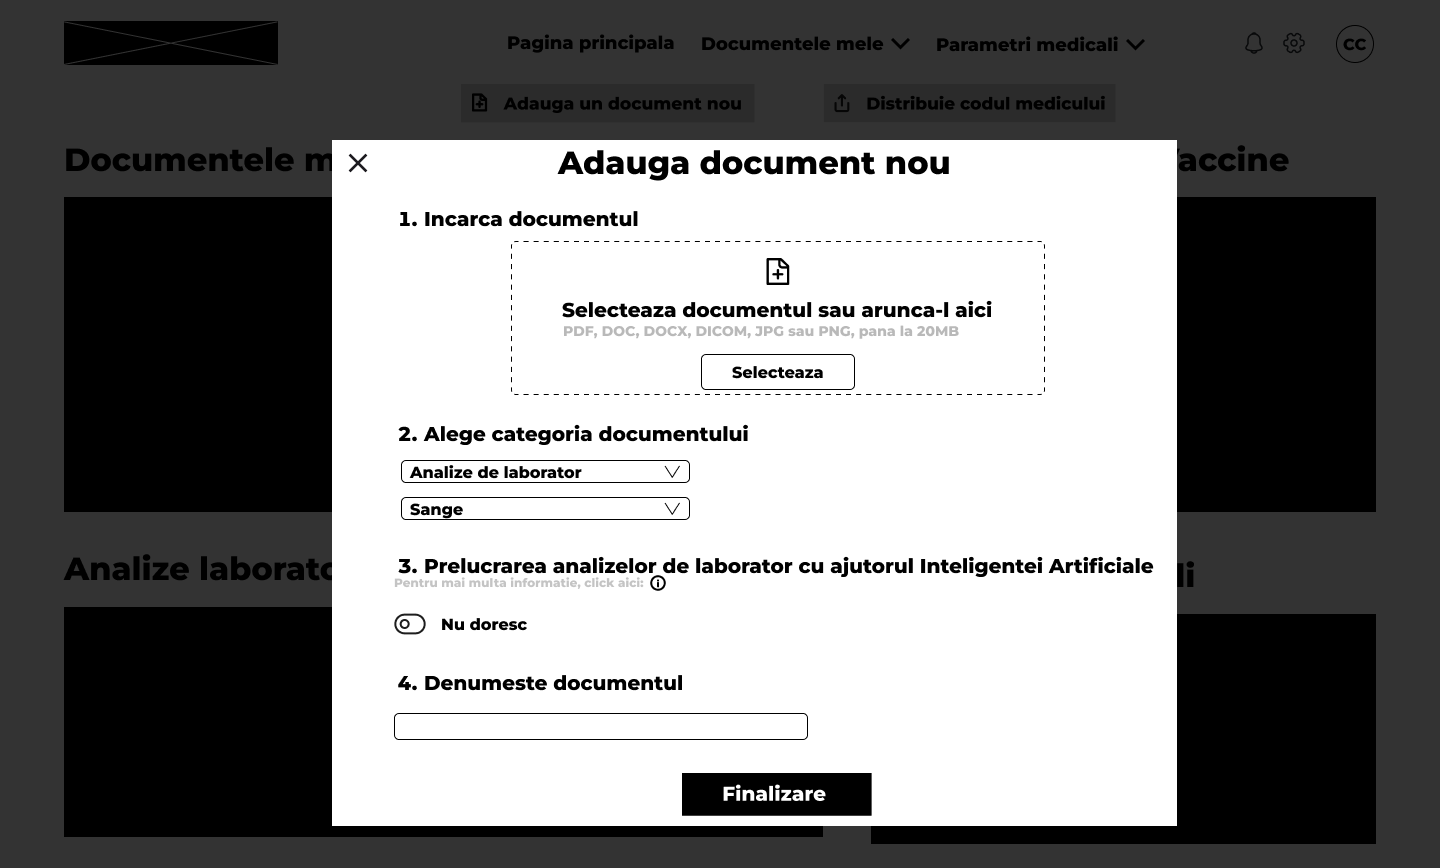
\includegraphics[width=0.70\textwidth]{wireframes/Desktop_newDoc.png}%
    }
    \hspace{0.05\textwidth}
    \subfloat[Mobile version]{%
        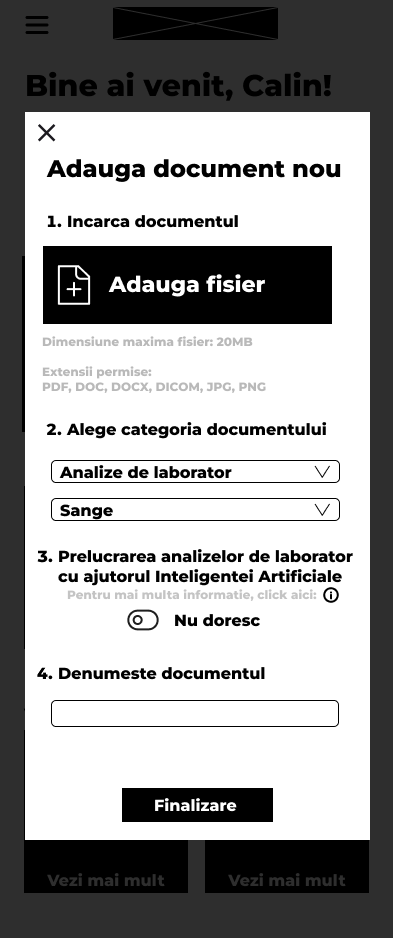
\includegraphics[scale=0.3]{wireframes/Mobile_newDoc.png}%
    }
    \caption{Desktop and Mobile version of the New Document screen}\label{fig:newDoc_wireframe}
\end{figure}

\begin{figure}[ht]
    \centering
    \subfloat[Desktop version]{%
        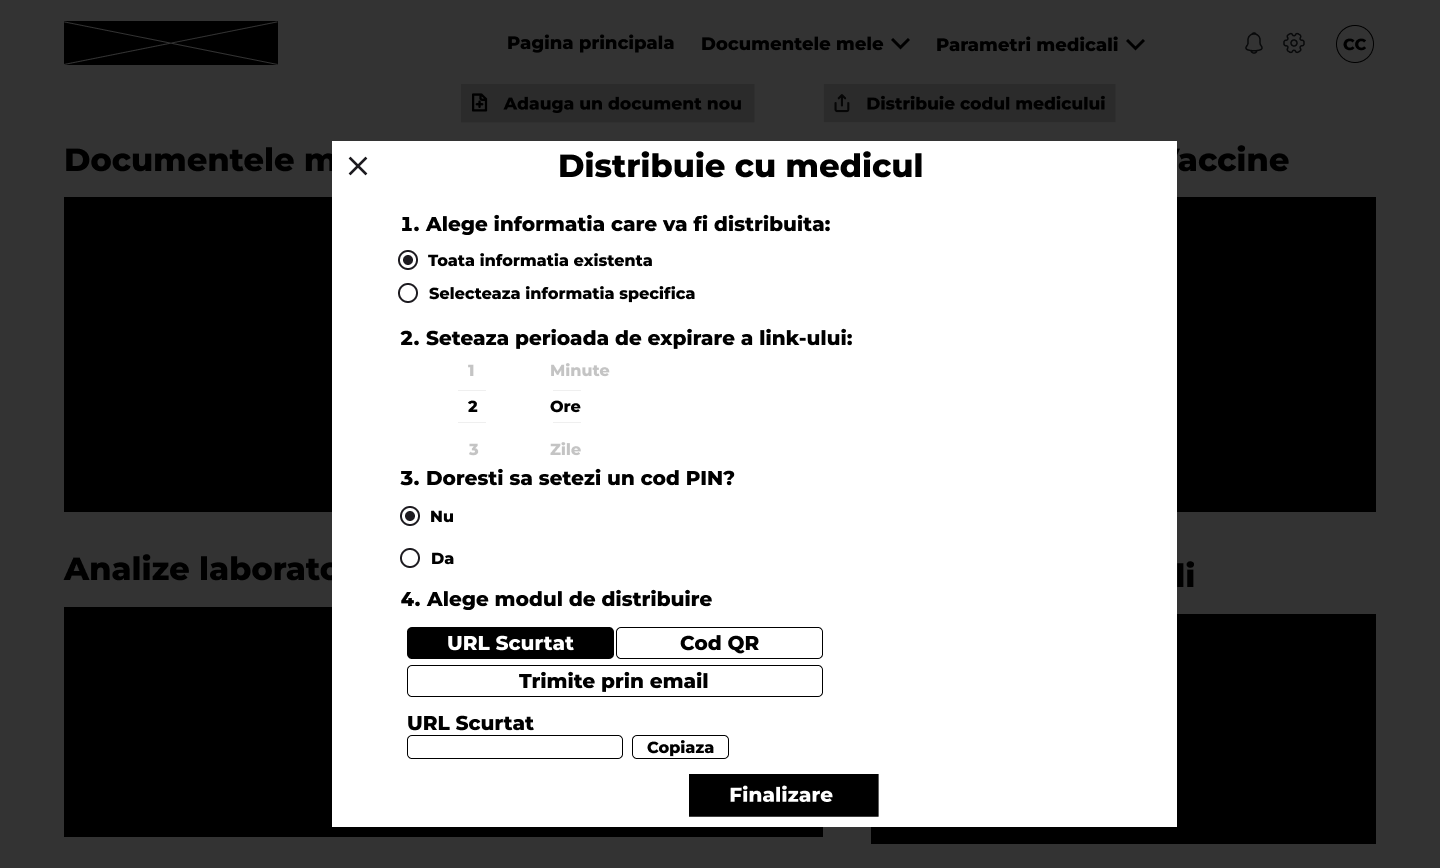
\includegraphics[width=0.75\textwidth]{wireframes/Desktop_shareDoctor.png}%
    }
    \hspace{0.05\textwidth}
    \subfloat[Mobile version]{%
        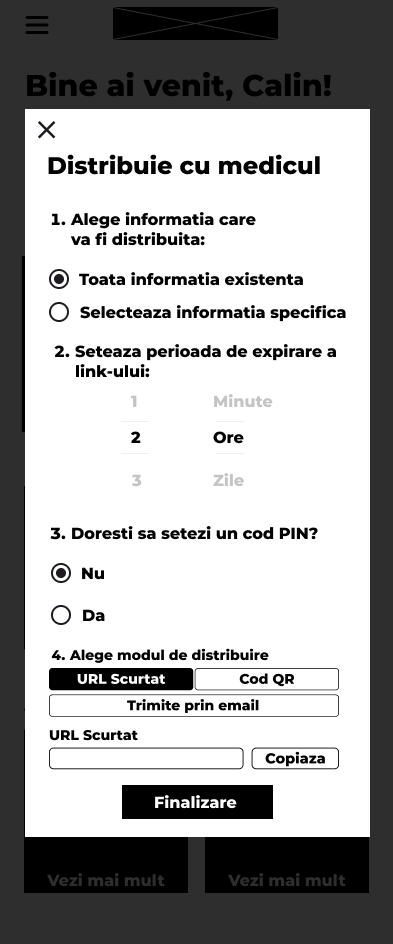
\includegraphics[scale=0.3]{wireframes/Mobile_shareDoctor.png}%
    }
    \caption{Desktop and Mobile version of the Share Doctor screen}
\end{figure}

\begin{figure}[ht]
    \centering
    \subfloat[Desktop version]{%
        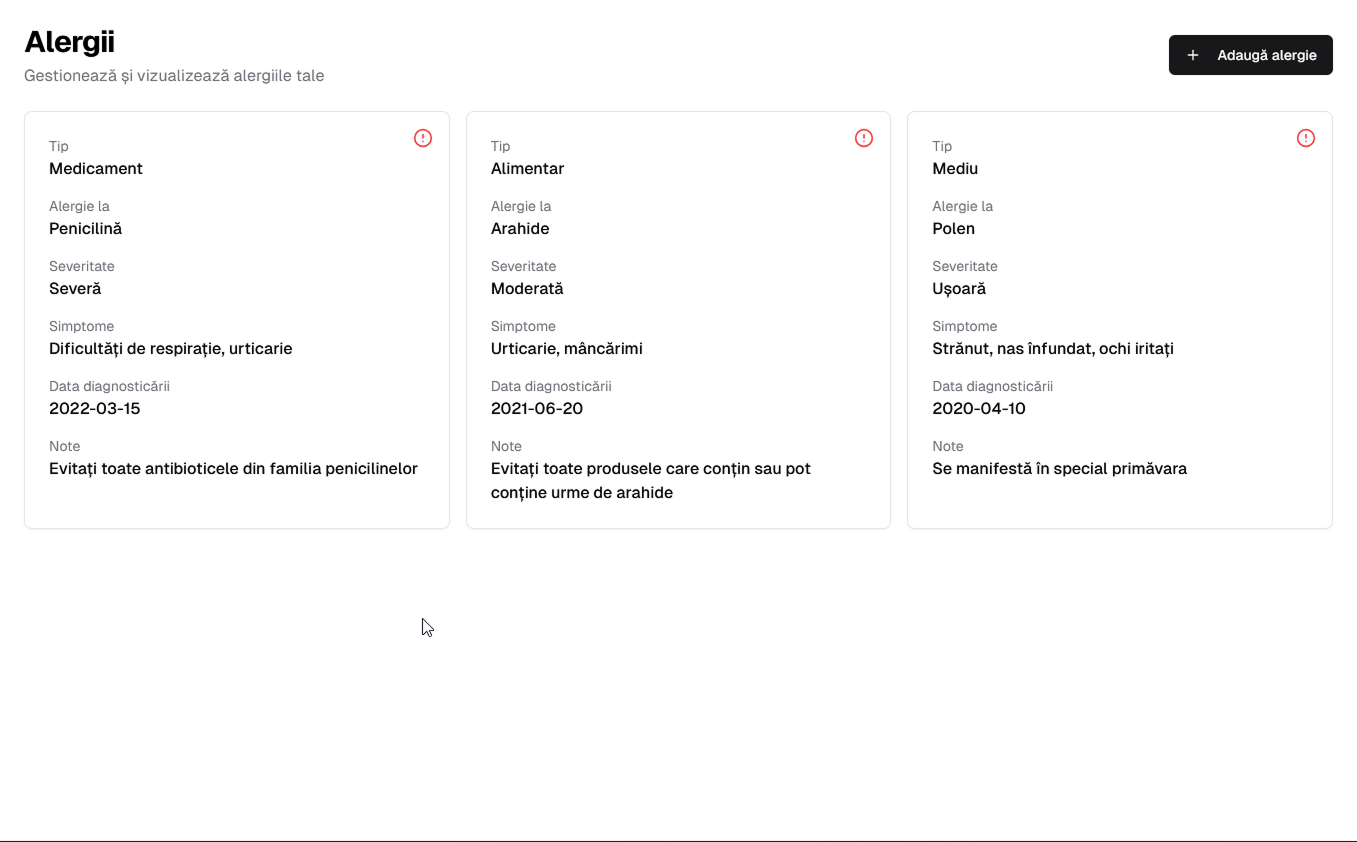
\includegraphics[width=0.75\textwidth]{wireframes/AI-allergies-desktop.png}%
    }
    \hspace{0.05\textwidth}
    \subfloat[Mobile version]{%
        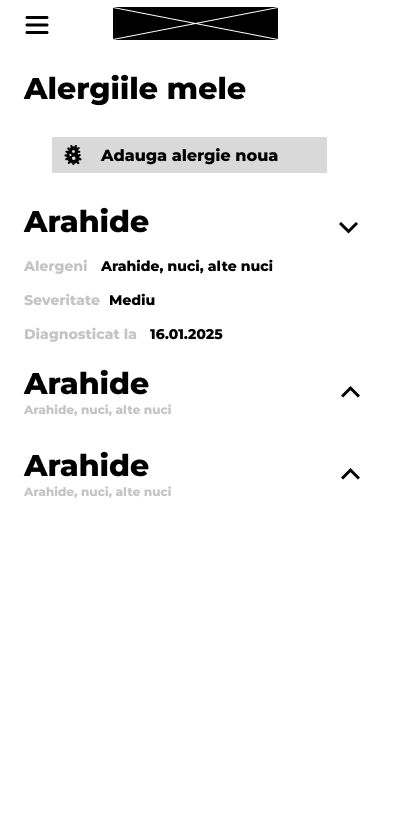
\includegraphics[scale=0.3]{wireframes/Mobile_allergies.png}%
    }
    \caption{Desktop and Mobile version of the Allergies screen}
\end{figure}

\chapter{Final Stakeholder Feedback}\label{sec:full_feedback}

Full feedback for stakeholder 1:

\begin{quotation}
`I appreciated the concept of the project and the way all essential components of a Personal Health Record were integrated: general, clinical, and paraclinical data, consultations, physician access, and data security. The platform is strongly patient-centered, enhancing access to personal medical data and significantly contributing to patient empowerment.

I would emphasize the importance of adhering to interoperability standards, both for future integration with hospital software systems and for enabling the upload of data from mobile devices.

From my perspective as a medical doctor specialized in public health and an expert in digital transformation of healthcare, I see great potential in this project and I am committed to offering the necessary support for its further development'
\end{quotation}

Full feedback for stakeholder 2:

\begin{quotation}
`I was really impressioned with the application on the digital health records book you have developed and presented to me. As a BA you have managed to capture the most important needs and then translated them into useful features included in the solution developed.

Even though it is one the first releases, it looks already complete and covers all the journey of a citizen fascinated with the use of the technology for managing the comprehensive records related to its health status in a very efficient and effective way. The application is user friendly, it looks so intuitive as the user can easily find any data or add something new to the app. It offers a lot of flexibility in terms of types of data that can be added and monitored. The dashboards and reports generated in the app are easy to read and understand, as well as provide insightful information on the evolution of the status. I also would like to mention the professional approach as you have provided for notifications related to personal data protection, as the applications seem to use very sensitive information.

By developing this solution you have given a new opportunity to Moldova to make one big step forward to the digitisation, and hope it will be largely used by moldovans as the country offers them also other related nice opportunities like high speed internet access and good coverage by 5G network'
\end{quotation}